%%%%%%%%%%%%%%%%%%%%%%%%%%%%%%%%%%%%%
%                                   %
% Compile with XeLaTeX and biber    %
%                                   %
% Questions or comments:            %
%                                   %
% joshua dot mcneill at uga dot edu %
%                                   %
%%%%%%%%%%%%%%%%%%%%%%%%%%%%%%%%%%%%%

\documentclass{beamer}
  % Read in standard preamble (cosmetic stuff)
  %%%%%%%%%%%%%%%%%%%%%%%%%%%%%%%%%%%%%%%%%%%%%%%%%%%%%%%%%%%%%%%%
% This is a standard preamble used in for all slide documents. %
% It basically contains cosmetic settings.                     %
%                                                              %
% Joshua McNeill                                               %
% joshua dot mcneill at uga dot edu                            %
%%%%%%%%%%%%%%%%%%%%%%%%%%%%%%%%%%%%%%%%%%%%%%%%%%%%%%%%%%%%%%%%

% Beamer settings
% \usetheme{Berkeley}
\usetheme{CambridgeUS}
% \usecolortheme{dove}
% \usecolortheme{rose}
\usecolortheme{seagull}
\usefonttheme{professionalfonts}
\usefonttheme{serif}
\setbeamertemplate{bibliography item}{}

% Packages and settings
\usepackage{fontspec}
  \setmainfont{Charis SIL}
\usepackage{hyperref}
  \hypersetup{colorlinks=true,
              allcolors=blue}
\usepackage{graphicx}
  \graphicspath{{../../figures/}}
\usepackage[normalem]{ulem}
\usepackage{enumerate}

% Document information
\author{M. McNeill}
\title[FREN2001]{Français 2001}
\institute{\url{joshua.mcneill@uga.edu}}
\date{}

%% Custom commands
% Lexical items
\newcommand{\lexi}[1]{\textit{#1}}
% Gloss
\newcommand{\gloss}[1]{`#1'}
\newcommand{\tinygloss}[1]{{\tiny`#1'}}
% Orthographic representations
\newcommand{\orth}[1]{$\langle$#1$\rangle$}
% Utterances (pragmatics)
\newcommand{\uttr}[1]{`#1'}
% Sentences (pragmatics)
\newcommand{\sent}[1]{\textit{#1}}
% Base dir for definitions
\newcommand{\defs}{../definitions}


  % Packages and settings

  % Document information
  \subtitle[Couleurs, comparatifs, superlatifs]{Les couleurs, les comparatifs et les superlatifs des adjectifs}

\begin{document}
  % Read in the standard intro slides (title page and table of contents)
  \begin{frame}
    \titlepage
    \tiny{Office: % Basically a variable for office hours location
Gilbert 121\\
          Office hours: % Basically a variable for office hours
 lundi, mercredi, vendredi 10:10--11:10
}
  \end{frame}

  \begin{frame}{}
    \begin{center}
      \Large Quiz
    \end{center}
  \end{frame}

  \begin{frame}{Comparons les couleurs}
    Avec un/e partenaire, comparez les couleurs de vos vêtements.
    Dis si tes vêtements sont \lexi{plus}, \lexi{moins} ou \lexi{aussi} colorés que les vêtements de ton/ta partenaire.
    \begin{columns}
      \column{0.5\textwidth}
        \begin{description}
          \item[] \textbf{Modèle:} \emph{chemise/chemisier/etc}
          \item[E1:] Ma chemise est plus bleue que ton teeshirt.
          \item[] \tinygloss{My shirt is more blue than your T-shirt.}
          \item[E2:] C'est vrai. Mon teeshirt est moins bleu que ta chemise.
          \item[] \tinygloss{That's true. My T-shirt is less blue than your shirt.}
        \end{description}
      \column{0.5\textwidth}
        \begin{enumerate}
          \item chemise / chemisier / \emph{etc}
          \item baskets / chaussures / \emph{etc}
          \item jean / jupe / pantalon / \emph{etc}
          \item casquette / chapeau / bonnet / lunettes
          \item anorak / veste / manteau / \emph{etc}
          \item chaussettes
          \item foulard / écharpe / cravate
        \end{enumerate}
    \end{columns}
  \end{frame}

  \begin{frame}[b]{Le superlatif}
    \only<2-3>{
      Qui est le plus grand? \underline{\uncover<3->{Riker est le plus grand. (6'4'')}}
    }
    \only<4-5>{
      Qui est le plus intelligent? \underline{\uncover<5->{Data est le plus intelligent. (Il est un androïde.)}}
    }
    \only<6-7>{
      Qui est le plus sympa? \underline{\uncover<7->{Troy est la plus sympa. (Elle est une empathe.)}}
    }
    \only<8-9>{
      Qui est le plus bleu? \underline{\uncover<9->{Guinan est la plus bleue.}}
    }
    \only<10-11>{
      Qui a les cheveux les plus roux? \underline{\uncover<11->{Crusher a les cheveux les plus roux.}}
    }
    \only<12-13>{
      Qui a les meilleures lunettes? \underline{\uncover<13->{Geordi a les meilleures lunettes.}}
    }
    \begin{center}
      \only<1>{
        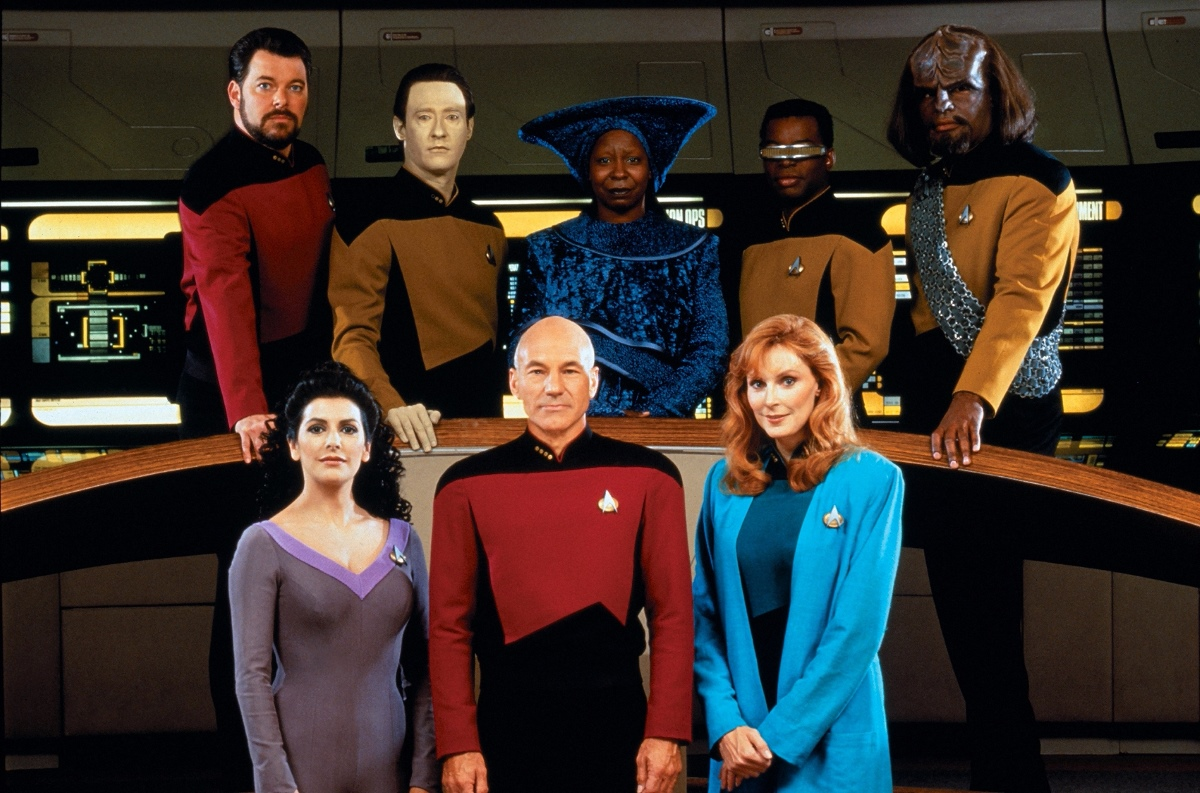
\includegraphics[scale=0.28]{star_trek.jpg}
      }
      \only<2->{
        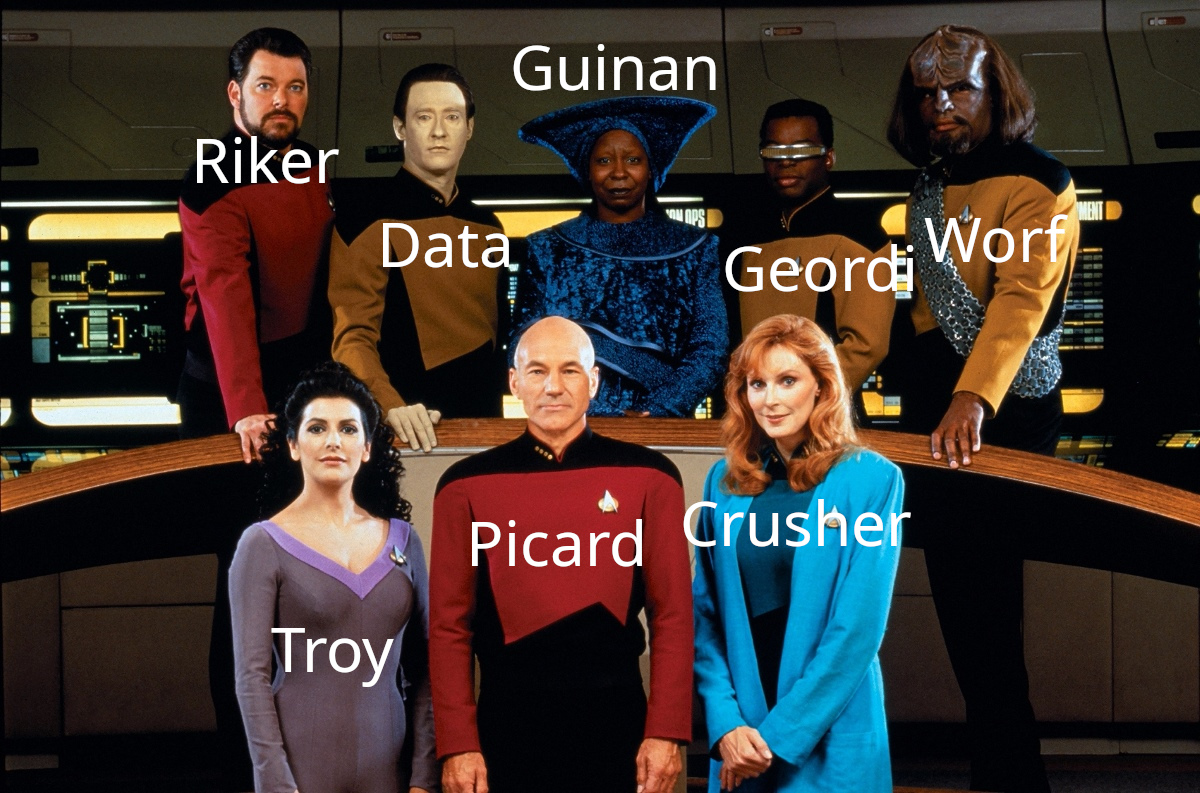
\includegraphics[scale=0.28]{star_trek_names.jpg}
      }
    \end{center}
  \end{frame}

  \begin{frame}{}
    En groupes de 3 à 5, discutez qui a les caractéristiques suivantes.
    Après, formez de nouveaux groupes est discutez les mêmes questions. \\
    \tinygloss{In groups of 3 to 5, discuss who has the following characteristics.
    After, form new groups and discuss the same questions.} \\
    \begin{description}
      \item[\textbf{Modèle:}] \emph{le/la plus grand/e?}
      \item[E1:] Qui est le plus grand ici?
      \item[E2:] Moi, je fais 5 pieds 4 pouces.
      \item[E3:] Et moi, je fais 6 pieds 5 pouces, alors je suis le plus grand.
    \end{description}
    \begin{columns}[t]
      \column{0.45\textwidth}
        \begin{enumerate}
          \item le/la plus grand/e?
          \item le/la plus jeune?
          \item le/la moins sérieux/-euse?
          \item le/la plus sociable?
          \item le/la plus ambitieux/-euse?
        \end{enumerate}
      \column{0.55\textwidth}
        \begin{enumerate}
          \setcounter{enumi}{5}
          \item le/la plus élégant/e?
          \item le/la moins doué/e pour le sport?
          \item le/la plus doué/e pour le français?
          \item le/la meilleur/e musicien/ne?
          \item le/la plus têtu/e?
        \end{enumerate}
    \end{columns}
  \end{frame}

  \begin{frame}{}
    \begin{center}
      \Large Questions?
    \end{center}
  \end{frame}
\end{document}
